% File              : notes.tex
%% Author            : Wayne Yeo [fishnsotong] <wwzyeo@gmail.com>
%% Date              : 2020-04-12T16:57:32+0800
%% Last Modified Date: 2020-08-31T06:49:19+0800
%% Last Modified By  : Wayne Yeo [fishnsotong@superheated] <wwzyeo@gmail.com>

\documentclass{article}

\usepackage{amsmath,amssymb,amsthm}
\usepackage[shortlabels]{enumitem}
\usepackage{physics}
\usepackage{titlesec}
\usepackage{tcolorbox}
\usepackage{achemso}
\usepackage{gensymb}
\usepackage{chemmacros}
  \chemsetup{modules={all}}

\usepackage{epigraph}
\setlength\epigraphwidth{10cm}

\usepackage{graphicx} %package to manage images
\graphicspath{ {images/} }

\hyphenpenalty=1000

\newtheorem{theorem}{Theorem}
\numberwithin{theorem}{section}
\newtheorem*{theorem*}{Theorem}
\newtheorem{corollary}{Corollary}
\numberwithin{corollary}{section}
\newtheorem*{corollary*}{Corollary}
\newtheorem{postulate}{Postulate}
\numberwithin{postulate}{section}
\newtheorem*{postulate*}{Postulate}
\newtheorem{lemma}{Lemma}
\numberwithin{lemma}{section}
\newtheorem*{lemma*}{Lemma}
\newtheorem{definition}{Definition}
\numberwithin{definition}{section}
\newtheorem*{definition*}{Definition}
\newenvironment{justification} {\begin{proof}[Justification]} {\end{proof}}


\titleformat
{\part} % command
[display] % shape
{\bfseries\Large\itshape} % format
{Part \ \thepart} % label
{0.5ex} % sep
{
    \rule{\textwidth}{1pt}
    \vspace{1ex}
    \centering
} % before-code
[
\vspace{-0.5ex}%
\rule{\textwidth}{0.3pt}
] % after-code

\DeclareMathOperator{\E}{\mathbb{E}}

\title{5.60 Thermodynamics and Kinetics}
\author{Wayne Yeo Wei Zhong}

\begin{document}

\maketitle

\begin{abstract}
  This course deals primarily with equilibrium properties of macroscopic
  systems, basic thermodynamics, chemical equilibirum of reactions in gas and
  solution phase, and rates of chemical reactions. Additional topics include
  electrochemistry, catalysis and enzyme kinetics.
\end{abstract}

\tableofcontents

\newpage

\section*{\centering{Useful Relations}}
\bigskip

\begin{equation*}
  \Delta_r G^{\standardstate} = -RT\ln{K}
\end{equation*}

\begin{equation*}
\Delta_r G^{\standardstate} = \Delta_r H^{\standardstate} - T \Delta_r S^{\standardstate}
\end{equation*}

\begin{equation*}
  E = E^{\standardstate'} + \frac{RT}{n'F} \ln{\frac{C_\mathrm{P}}{C_\mathrm{Q}}}
\end{equation*}
\newpage

\part{Thermodynamics}

\epigraph{[\textbf{Thermodynamics} is] the only physical theory of universal
content concerning which I am convinced that, within the framework of the
applicability of its basic concepts, it will never be overthrown.}{Einstein}

The systematic, quantitative discussion of the transfer and transformation of
energy in bulk matter is called thermodynamics. The primary objective of
chemical thermodynamics is the establishment of a criterion to determine the
feasibility or spontaneity of a given transformation. Some examples of processes
that we consider are chemical reactions, phase changes and the formation of
solutions. 

The effectiveness of thermodynamics can be explained by the certain distinctions we
make about what the system is. The
\textbf{thermodynamic system} is a precisely defined region of the universe
under study. Everything in the universe except the system is called the
surroundings.

The thermodynamic description of these chemical systems employ the \textbf{laws
of thermodynamics}, that form an axiomatic basis. The first law specifies that
energy can be exchanged between physical systems as heat and work.
The second law defines the existence of a quantity called entropy, that
describes the thermodynamic direction in which the system can evolve.

The entropy of a system is of particular interest to us when studying chemical
systems, as it enables us to identify the spontaneous direction of a chemical
reaction, and the composition of a system when the reaction is at equilibrium.

Later in the course, we will be introduced to \textbf{statistical mechanics},
where we will come to understand the relationship between molecular and bulk
properties. The quantization of energy to discrete levels will play an
increasingly important role at the molecular scale, where we consider
rotational, vibrational and electronic modes of motion.

In conclusion, thermodynamics resides at the heart of phyiscal chemistry. We
consider whether chemical processes \textit{can happen}, and \textit{to what
extent} they happen. It is important to note that thermodynamics remains silent
regarding \textit{how fast} they occur, which will
be dealt with in kinetics at a later stage.

\setcounter{section}{0}
\section{States, equations of state, 0th law}

\subsection{Laws of thermodynamics}

\paragraph{0th law of thermodynamics.} If $A$ and $B$ are in thermal equilibrium
and $B$ and $C$ are in thermal equilibrium, then $A$ and $C$ are in thermal 
equilibrium. \textit{Defines Kelvin scale.}

\paragraph{1st law of thermodynamics.} $U$ is conserved. \textit{You can break
even.}

\begin{equation}
  \mathrm{d}w + \mathrm{d}q = \mathrm{d}U
\end{equation}

\paragraph{2nd law of thermodynamics.} Defines entropy and the direction of
time. \textit{You can break even at 0 K}.

\begin{equation}
  \Delta S = \int \frac{\textnormal{d} q_{\mathrm{rev}}}{T}
\end{equation}

\paragraph{3rd law of thermodynamics.} Defines the absolute scale of $T$. For
pure crystal, $S \rightarrow 0$ as $T \rightarrow 0$. \textit{You can never
reach 0 K}.

\subsection{Definitions}

\subsubsection{Types of systems}
\begin{itemize}
  \item Open systems (free transfer of energy and matter).
  \item Closed systems (free transfer of energy, but not matter).
  \item Isolated systems (no transfer of energy and matter).
\end{itemize}

\subsubsection{Types of properties}
\begin{itemize}
  \item{Intensive properties (temperature, molar volume, molar mass, density)}
  \item{Extensive properties (mass, volume, pressure)}
\end{itemize}

To get an intensive property from an extensive property, divide the property by
its molar amount.

\subsection{Properties of gases}

\paragraph{Kelvin scale of temperature. }
\begin{equation}
  T(\mathrm{K}) = \theta (\mathrm{\degree C}) + 273.15
\end{equation}

\subsection{Equations of state for ideal gases}

\paragraph{Ideal gas law. }
\begin{equation}
  pV = nRT
\end{equation}

This is an example of an equation of state $V = f(n, p , T)$

\subsection{Equations of state for non-ideal gases}

\subsubsection{Compressibility factor $Z$}

At high pressures molecules are colliding more often. This allows repulsive
forces between molecules to have a noticeable effect, making the molar volume of
the real gas  greater than the molar volume of the corresponding ideal gas,
making $Z > 1$. When pressures are lower, the molecules are free to move. In this case
attractive forces dominate, making $Z < 1$.

\begin{equation}
  p \overline{V}_\mathrm{real} = ZRT
\end{equation}

\begin{equation*}
  Z = \frac{\overline{V}_\mathrm{real}}{\overline{V}_\mathrm{ideal}}
\end{equation*}

\subsubsection{Virial expansion}

Typically expresses pressure $p$ as a power series in number density. The virial coefficients are empirically determined(?) and can be looked up in tables.

\begin{equation}
  \frac{p \overline{V}}{RT} = Z(T) = 1 + \frac{B(T)}{\overline{V}} +
  \frac{C(T)}{\overline{V}^2} + ...
\end{equation}

As $p \rightarrow 0$, $\overline{V} \rightarrow \infty$, a real gas
approaches the behaviour of an ideal gas.

\subsubsection{van der Waals equation of state}

An extension of the ideal gas equation to account for intermolecular interactions,
where $\overline{V}$ denotes molar volume. It only has two parameters, and is
thus very useful. The factor $b$ accounts for the volumes that gas particles
occupy as hard spheres.

\begin{equation}
  \left( p + \frac{a}{\overline{V}^2} \right) (\overline{V} - b) = RT 
\end{equation}

Notice that Equation 4 reduces to $pV = nRT$ when $\overline{V}$ is large.

\section{Work, heat, first law}

\subsection{Work}

\paragraph{Sign convention. }Contra to engineering, chemical science adopts
a sign convention that is \textit{additive} in nature. $q$ represents the heat
absorbed \textit{by} the system, and $w$ represents work done \textit{on} the
system.

\paragraph{Expansion work of a gas at constant external pressure.} Because
external pressure is constant, this equation is for irreversible processes.

\begin{equation}
  \delta w' = p_{\mathrm{ext}} \mathrm{d}V
\end{equation}

\begin{justification}
  The force which the system moves against is due to the \textit{external
  pressure}. For a piston with area $A$, the force on the piston is $p_{ext}A$. If the
  piston moves out by a small distance $\mathrm{d}x$.

  \begin{equation*}
  \begin{split}
    \delta w' & = F\mathrm{d}x \\
    & =  p_{ext} A \mathrm{d}x \\
    & = p_{ext} \mathrm{d}V
  \end{split}
\end{equation*}

\end{justification}

It might be counter-intuitive to consider \textit{external} pressure as the
quantity that determines the work doen by the gas when it expands. This seems
odd, surely it is the gas inside the cylinder that is 'doing the pushing.' And
so, the force which is doing the work is that provided by the gas inside the
cylinder.

The work done \textit{by the system} depends crucially on what the system is. If
the system is defined to be a gas in a cylinder with a piston, it is the gas
that expands against the surrounding pressure. It is then clear that the force \textit{against which the system pushes} is that
supplied by the external pressure.

It's certainly true that the gas only expands if the internal pressure exceeds
the external pressure. However, when the external pressure is zero, the system does no work as it expands,
because it has nothing to push against. This is a \textbf{free expansion}.

\paragraph{Expansion work of a gas against variable external pressure. }If
$p_\mathrm{ext}$ is not constant, then we have to look at infinitesimal
changes.

\begin{equation}
  w = - \int_{V_i}^{V_f} p_\mathrm{ext} \mathrm{d}V
\end{equation}

\subsubsection{Reversible changes}

Expansions where $p = p_\mathrm{ext}$. That is, adjusting hypothetical weights on the
piston as the gas is expanding to ensure the above condition. This is to ensure
that $p_{ext}$ is infinitesimally smaller than $p$ at each step of the process.
In conclusion, \textit{maximum work} is done when an expansion is reversible, as the external
pressure which determines the work done is inifinitesimally smaller tham the
internal pressure.

\paragraph{Reversibility. }At any point a reversible expansion can be turned into
a compression simply by making the external pressure infinitesimally greater
than the internal pressure. As the internal and external pressures are only
infinitesimally different, the system can be considered always in balance; it
could go both ways! Thus, we can say that reversible processes are also
\textit{equilibrium processes.}

\subsection{The path dependence of $w$ and $q$}

\subsubsection{Work depends on the path}

\paragraph{Example. }Let us assume a reversible process for such that $p =
p_\mathrm{ext}$,

\begin{equation*}
  \mathrm{Ar} (\mathrm{g}, p_1, V_1) = \mathrm{Ar} (\mathrm{g}, p_2, V_2)
\end{equation*}

A compression occurs such that $V_1 > V_2$ and $p_1 < p_2$. There are two
possible paths that can achieve the same result, as seen in Fig. 1.

\begin{figure}[h]
\caption{Two different paths for the same change in state}
\centering
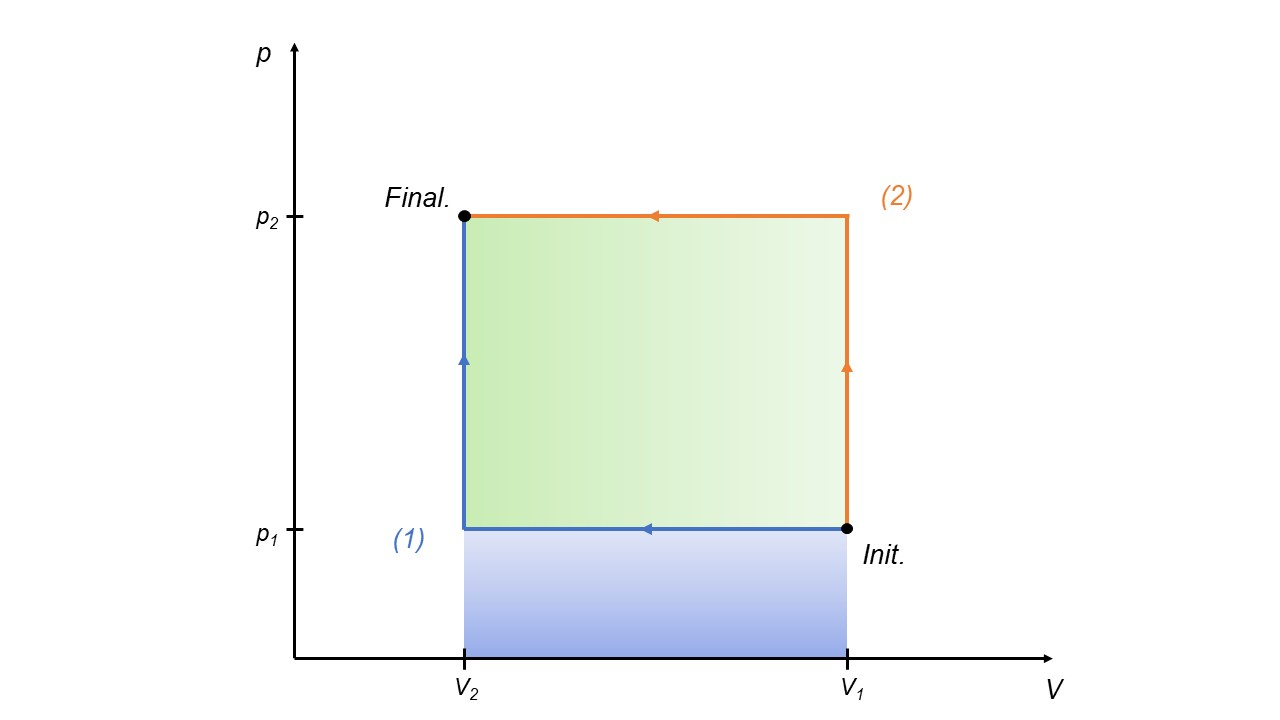
\includegraphics[width=1.0\textwidth]{fig1.jpg}
\end{figure}



\paragraph{Work. }As we've seen in the example of a heat engine above, work is \textbf{not} a
function of state, and is path dependent. For a cyclic process where the system returns to the initial state, it is
possible for $\oint \mathrm{d} w \neq 0$.

\paragraph{Heat. }Transfer of energy between the system and surroundings that
can be used to raise the temperature of the system.

\paragraph{Heat capacity $C$. }Connects heat with temperature. 

\begin{justification}

  \begin{equation}
    \delta q = C_\mathrm{path} \mathrm{d}T \qquad \mathrm{or} \qquad C_\mathrm{path} = \left( \frac{\delta q}{\mathrm{d} T} \right)_\mathrm{path}
  \end{equation}

  If $C$ is path-dependent, as we can see from the presence of different heat capacities for
  constant volume ($C_v$) and constant pressure ($C_p$), then heat is also a
  path-dependent quantity, as shown below.

  \begin{equation*}
    q = \int_\mathrm{path} C_\mathrm{path} \mathrm{d} T
  \end{equation*}

\end{justification}

Heat capacity is surprisingly important, we will come back to it in further
detail at a later section.

\subsubsection{The equivalence of work and heat}

Experimentally, it was found that

\begin{equation*}
  \oint (\delta q + \delta w) = 0
\end{equation*}

This implies that the sum $(q + w)$ is independent of the path. We
can thus deduce that there is a \textit{state function} whose differential is
$\delta q + \delta w$.

This is very surprising, how can a path-independent state function emerge from
two path-dependent variables?

\subsection{The First Law of Thermodynamics}

\begin{definition}[First Law of Thermodynamics]
The internal energy $\Delta U$ changes only when a system takes up or gives off
heat $q$ or work $w$.

  \begin{equation}
    \Delta U = q + w
  \end{equation}
\end{definition}

This is a statement of the equivalence of heat and work. The internal energy of
an isolated system is constant; if $\Delta U$ increases in the system, the
energy decreases in the surroundings.

\begin{corollary}[Clausius Statement of the First Law]
  As the internal energy of an isolated system is constant, an increase in
  $\Delta U$ in the system would lead to an energy decrease of the same
  magnitude in the surroundings.

  \begin{equation*}
    \Delta U_\mathrm{system} = q + w \qquad \Delta U_\mathrm{surroundings} = - q - w
  \end{equation*}

  \begin{equation}
    \implies \Delta U_\mathrm{universe} = \Delta U_\mathrm{system} + \Delta
    U_\mathrm{system} = 0
  \end{equation}

\end{corollary}
The energy of the universe is conserved.

\section{Internal energy, expansion work}

\subsection{Isothermal gas expansion ($\Delta T = 0$)}

\subsubsection{Isothermal, reversible expansions}

\paragraph{Work done in an isothermal, reversible expansion. }

\begin{equation}
  w' = nRT\ln{\frac{V_f}{V_i}}
\end{equation}

\paragraph{Entropy change for isothermal expansions. }

\begin{equation}
  \Delta S = nR \ln{\frac{V_f}{V_i}}
\end{equation}

\begin{justification}
  For an isothermal system, $\Delta U = 0$. According to the \textbf{First Law
  of Thermodynamics}, $-w = q$. Thus, we can see that
  \begin{equation*}
      q = nRT\ln{\frac{V_f}{V_i}}.
  \end{equation*} Which can be rearranged to give $\Delta S$. Because $S$ is a
  state function and is independent of the path taken, the expression below is
  valid regardless of the reversibility of the expansion.
\end{justification}

\subsection{The internal energy $U$}

\subsubsection{Heat capacity}

\subsubsection{Joule free expansion of an ideal gas}

\begin{tcolorbox}
  The internal energy of an ideal gas depends only on temperature
\end{tcolorbox}


\section{Enthalpy}

Chemical reactions and biological processes typically occur under
\textbf{constant pressure} and with \textbf{reversible $pV$ work}. Enthalpy
turns out to be an especially useful state function under those conditions.

\subsection{The definition of $H$ }

\begin{definition}
  Enthalpy is the sum of a system's internal energy and the product of its pressure and
  volume. The heat absorbed or released by closed systems at constant pressure
  equals the change in enthalpy.
  \begin{equation}
   H := U + pV
  \end{equation}
\end{definition}

Though this definition may seem arbitrary, a result of consequence is the heat
absorved or released by closed systems at constant pressure equals the change in
enthalpy of the system.

\begin{justification}
  By definition, $H = U + pV$. As the system undergoes a small change of $\mathrm{d}H$,
  \begin{equation*}
    \begin{split}
      H + \mathrm{d}H & = U + \mathrm{d}U + (p + \mathrm{d}V)(V + \mathrm{d}p) \\
      & = U + \mathrm{d}U + pV + p\mathrm{d}V + V\mathrm{d}p +
      \mathrm{d}p\mathrm{d}V
    \end{split}
  \end{equation*}
  As the product of two infinitesimal equations can be neglected,

  \begin{equation*}
    \begin{split}
      H + \mathrm{d}H & = H + \mathrm{d}U + V\mathrm{d}p + p\mathrm{d}V \\
      \mathrm{d}H & = \mathrm{d}U + V\mathrm{d}p + p\mathrm{d}V
    \end{split}
  \end{equation*}
  
  Which is known as the \textit{complete differential} of the definition of
  enthalpy.

  By the \textbf{First Law of Thermodynamics} $\mathrm{d}U = \mathrm{d}q +
  \mathrm{d}w$, the term $\mathrm{d}w = -p\mathrm{d}V$ can be substituted into
  the complete differential as a system under mechanical equilibrium does only
  expansion work.
  
  \begin{equation*}
    \begin{split}
      \mathrm{d}H & = \mathrm{d}U + V\mathrm{d}p + p\mathrm{d}V \\
      & = \mathrm{d}q - p\mathrm{d}V + V\mathrm{d}p + p\mathrm{d}V \\
      & = \mathrm{d}q + V\mathrm{d}p
    \end{split}
  \end{equation*}

Finally, the condition of \textit{constant pressure} is imposed on the system, which is the case for most chemical changes even in a practical sense. This means that $V\mathrm{d}p = 0$. Which gives,

\begin{equation}
  \mathrm{d}H = \mathrm{d}q_{\mathrm{const. pressure}}
\end{equation}

\end{justification}

From the above justification, we can see why $H$ is a good measure of the energy
transferred as heat in the various bond-forming and bond-breaking
transformations that we encounter in chemistry, which we often invoke in
thermochemical calculations.

\subsection{Joule-Thomson expansion}

\section{Adiabatic changes}

\textbf{Adiabatic processes} occur without transfer of energy as heat.

\section{Thermochemistry}

\section{Calorimetry}

\section{The Second Law of Thermodynamics}

\pagebreak

\section{Entropy and the Clausius inequality}

A key aim of physical chemistry is to seek a physical principle or law which
determines which processes will be spontaneous, and which will not. A tempting
idea is that reactions are spontaneous because the products are \textit{more
stable} than the reactants, which implies that they are lower in energy.
However, we can think of examples where processes are spontaneous but are
\textit{not} exothermic. 

Thus, energy minimization is \textit{not} the criterion for spontaneous
processes. This leads to a necessary discussion on the \textbf{Second Law of
Thermodynamics}.

\subsection{Microsopic view of entropy}

\paragraph{Boltzmann distribution. } The most probable distribution of a
particular system. $W$ represents the number of possible configurations of a
system.

\begin{equation}
  S = k_{B} \ln{W}
\end{equation}

We can consider a few factors that increases $S$ by increasing $W$. In fact, most
macroscopic principles regarding entropy can be rationalized as such.

\begin{itemize}
  \item \textit{Supplying energy as heat:} increases $W$ and hence increases the
    entropy.
  \item \textit{Increasing volume:} increasing the number of energy levels
    available, which increases $W$, which
\end{itemize}

The chief reason behind abandoning these definitions and their consequences for
empirical laws is practical in nature, and helps with understanding and
manipulating their effects on bulk matter. We will return to this statistical
understanding on entropy in \textit{statistical mechanics} at a later time.

\begin{definition}[Second Law of Thermodynamics]
  In a spontaneous process, the entropy of the Universe increases
\end{definition}

\section{Entropy and irreversibility}

We've now discussed both entropy and reversible processes separately, now we
will consider how the disorder of a system affects whether a process is
spontaneous, reversible or entirely impossible.

\section{Fundamental equation, absolute $S$, third law}

\subsection{The Master Equation}

\section{Criteria for spontaneous change}

\section{Gibbs free energy}

\section{Helmholtz free energy}

\section{Multicomponent systems, chemical potential}

\section{Chemical equilibrium}

\section{Temperature, pressure and $K_p$}

\section{Equlibrium: application to drug design}

Our analysis of equilibrium typically involves breaking and forming covalent
bonds. Thus, they apply equally well to bio-organic reactions, such as those
involved in ligand-receptor binding.

\section{Phase equilibria}

\subsection{Properties of pure substances}

\subsection{Clausius-Clapyreon equation}

\subsection{Properties of mixtures}

\subsubsection{Ideal solutions}

\subsubsection{Non-ideal solutions}

\subsection{Colligative properties}

\section{Introduction to statistical mechanics}

\section{The partition function}

\subsection{$q$, large $N$ limit}

\subsection{$Q$, many particles}

\section{Statistical mechanics and discrete energy levels}

\section{Model systems}

\section{Applications: chemical and phase equilibria}

\part{Kinetics}

\section{Introduction to reaction kinetics}

\subsection{Defining reaction rate}

\paragraph{Reaction rate.} For a given reaction $\mathrm{aA} + \mathrm{bB}
\rightarrow \mathrm{cC} + \mathrm{dD}$, the reaction rate is

\begin{equation}
  -\frac{1}{\mathrm{a}} \frac{\mathrm{d[A]}}{\mathrm{d}t} 
\end{equation}

\paragraph{Half-life.} $t_{1/2}$ is the time at which $[\mathrm{A}] =
0.5[\mathrm{A}]_0$.


\section{Complex reactions and mechanisms}

\section{Steady-state and equilibrium approximations}

\subsection{Pre-equilibrium approximation}

\subsection{Steady-state approximation}

\section{Chain reactions and explosions}

\section{Temperature, $E_a$, catalysis}

\paragraph{Dependence of rate on temperature. }The rate constant generally
depends quite strongly on temperature. Experimental studies have show that this
temperature dependence often follows the \textit{Arrhenius equation.}

\begin{equation}
  k = A \mathrm{exp} \left( \frac{- E_a}{RT} \right)
\end{equation}

\section{Enzyme catalysis}

\section{Autocatalysis and oscillators}

\subsection{Outlook}

With this, we conclude the main part of this course. Now, you are free to
proceed to the elective parts at the end, which include electrochemistry and
photochemistry. As these sections mature, I'm planning to transfer them to their
own document, where they can be given undivided attention to.

\textit{What's after all this?} Now, you're more than well equipped to tackle
the question of why chemical reactions happen. If you're more interested in the
fundamental nature of chemistry, the microscopic properties of its building
blocks and their electronic structure, I highly recommend you check out
\textit{5.61 Physical Chemistry}, which gives a complete treatment of molecular
quantum mechanics that is beyond the scope of this course.

Alternatively, should you wish to take a deeper look into statistical mechanics,
you could check out some of the textbooks on the subject (the one by Garland
Science is pretty good). A set of course notes should soon appear on this topic.

If you're interested in the topics presented in this final section, including
autocatalysis and oscillators, there are many more things you can look into. For
example,

\begin{itemize}
  \item Belousov–Zhabotinsky reaction
  \item Non-equlibrium thermodynamics
  \item Molecular switches, machines and replicators
\end{itemize}

All of which will be the subject of another exciting series of notes.

\part{Electrochemistry}

\section{Introduction to electrochemistry}

A simple example of energy storage is the \textbf{capacitor}. Capacitance is
defined as a constant

\begin{equation}
  C = \frac{Q}{V_c}.
\end{equation}

The current is

\begin{equation}
  I = -\frac{\mathrm{d}Q}{\mathrm{d}t} = -C \frac{\mathrm{d}V_c}{\mathrm{d}t}.
\end{equation}

Capacitors in general, fail as an energy storage device due to their lower
specific energy compared to batteries. However, they do have a number of
compelling properties. Storing power as electrical charge rather than chemical
potential has its benefits: this typically allows near instant charge times, and
very high peak output currents. In addition, they can survive many more (around
by a factor of ~$10^3$!) more charge-discharge cycles than fully-cycled
batteries.

\section{The electrochemical cell}

\section{Potentials, interfaces, electrodes and mass transport}

\section{Heterogeneous electron transfer}

\subsection{Tafel equation}

\subsection{Butler-Volmer equation}

\section{Dynamic electrochemical techniques}

\section{Electrochemical energy storage}

\subsection{Batteries}

\subsection{Fuel cells}

\subsection{Supercapacitors and electrode storage}

\section{Analytical methods in electrochemistry}

\subsection{Electrochemical methods}

\subsubsection{Electrochemical impedance spectroscopy}

\subsubsection{Cyclic voltammetry}

\subsubsection{Catalytic peak current analysis}

\subsubsection{Foot-of-the-wave analysis}

\subsubsection{Peak shift analysis}

\subsection{Complementary spectroscopic methods}

\subsubsection{Spectroelectrochemistry}

\subsubsection{Stopped-flow rapid mixing}

\subsubsection{Transient absorption spectroscopy}

With time-resolved spectroscopy, we can study dynamic processes in materials or
chemical compounds by means of spectroscopic techniques.



\end{document}
